\chapter{Modello ISO-OSI}
Ad oggi internet è il più grande sistema ingegneristico mai creato dall'umanità, che 
comprende miliardi di utenti e macchine.

\noindent Le operazioni chiave nella rete sono:
\begin{itemize}
    \item invio e consegna di pacchetti 
    \item instradamento dei pacchetti 
    \item individuazione degli indirizzi
\end{itemize}

\section{Protocolli}
Sono un \textbf{insieme formale di regole} durante un'interazione; descrivono come i computer trasmettono 
i dati attraverso una rete, come il formato e l'ordine dei messaggi, oltre alle azioni intraprese sulla 
trasmissione e/o ricezione di essi.

\section{Layering}
Per far fronte alla complessità, i protocolli sono organizzati in uno \textit{stack} di livelli

$\rightarrow$ i dati vengono passati dal livello più alto a quello più basso 

\noindent Questo facilita la manutenzione e l'aggiornamento del sistema.

\begin{figure}[H]
    \centering
    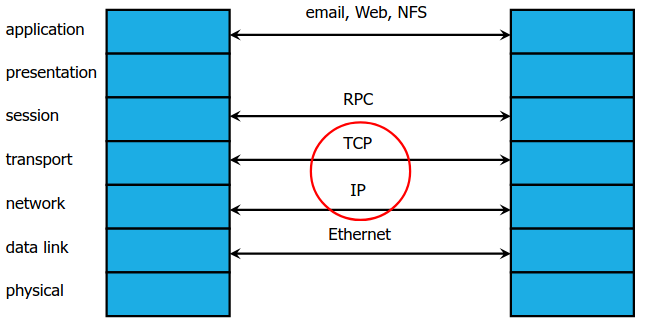
\includegraphics[width=1\linewidth]{chapters/7/images/osi-stack.png}
    \caption{OSI stack}
\end{figure}

\section{Principio end-to-end}
Le funzionalità specifiche dell'applicazione risiedono nei nodi finali di comunicazioni della rete, 
piuttostoc che nei nodi intermedi come \textit{gateway} e \textit{router}; l'\textit{intelligenza}
sta ai vertici della rete.

\section{Tipi di indirizzi in Internet}

\begin{itemize}
    \item \textbf{MAC} nel livello di accesso alla rete 
    \begin{itemize}
        \item associata alla scheda con interfaccia di rete 
        \item 48/64 bit 
    \end{itemize}
    \item \textbf{IP} per il livello di rete 
    \begin{itemize}
        \item 32bit per IPv4, 64bit per IPv6
        \item Ad esempio, 128.3.23.3
    \end{itemize}
    \item \textbf{IP + porte} per il livello di trasporto
    \begin{itemize}
        \item Ad esempio, 128.3.23.3:80
    \end{itemize}
    \item \textbf{Dominio} per livello di applicazione/umano 
    \begin{itemize}
        \item Ad esempio, www.inter.it 
    \end{itemize}
\end{itemize}

\subsection{Routing e traduzione degli indirizzi}
\begin{itemize}
    \item Routing tra indirizzi IP ed indirizzi MAC 
    \begin{itemize}
        \item protocollo di risoluzione degli indirizzi (ARP) per IPv4 
        \item Neighbour Discovery Protocol (NDP) per IPv6
    \end{itemize}
    \item Routing con indirizzi IP 
    \begin{itemize}
        \item TCP, UDP, IP per instradare pacchetti 
        \item Border Gateway Protocol per gli aggiornamenti delle tabelle di routing 
    \end{itemize}
    \item Traduzione da indirizzi IP a nomi di dominio 
    \begin{itemize}
        \item DNS
    \end{itemize}
\end{itemize}

\section{Interfaccia di rete}
Un computer può avere più interfaccie di rete; i pacchetti vengono trasmessi tra le interfacce 
di rete.



\noindent Impara l'indirizzo MAC di ogni computer ad esso connesso ed inoltra i frame solo al 
computer di destinazione.

\section{Netmask}
La netmask è una sequenza di 32 bit che identifica quali bit sono comuni negli indirizzi IP 
all'interno di una LAN (sottorete).

Ad esempio, 159.132.30.0/24 $\rightarrow$ 24 bit per la sottorete

\section{Tipi di minacce nella rete}
\begin{itemize}
    \item Confidenzialità (\textit{packet sniffing})
    \item Integrità (\textit{session hijacking})
    \item Disponibilità (DoS)
    \item \textit{Translation poisoning, routing}
\end{itemize}

\newpage
\section{ARP (Address Resolution Protocol)}
Il protocollo ARP connette il livello di rete con il livello dati, \textbf{convertendo un 
indirizzo IP in un indirizzo MAC}.

\noindent Ogni nodo mantiene una tabella (\textit{ARP cache}) in cui ci sono le associazioni 
già note; altrimenti, si chiede a tutti i nodi della rete locale chi ha un certo indirizzo IP.

$\rightarrow$ ARP funziona inviando $n$ messaggi broadcast e memorizzando nella cache le risposte, per utilizzi futuri:
\begin{itemize}
    \item \textit{ARP request} (effettuata in broadcast)
    \begin{itemize}
        \item \texttt{who has <IP1> tell <IP2>} 
    \end{itemize}
    \item \textit{ARP reply}
    \begin{itemize}
        \item \texttt{<IP1> is <MAC>}
    \end{itemize}
\end{itemize}

\subsection{ARP spoofing - Cache poisoning}
Viene fatta una \textit{assunzione di trust} nella LAN, dato che:
\begin{itemize}
    \item le richieste non vengono tracciate 
    \item gli annunci non sono autenticati 
    \item le macchine si fidano una dell'altra 
\end{itemize}

$\rightarrow$ una macchina malevola puà ingannare le altre 

\noindent Dato che una \textit{cache ARP} si aggiorna ogni volta che riceve una risposta ARP anche 
se non ha inviato alcuna richiesta \dots è possibile \textit{avvelenare} una cache inviando delle 
risposte \textit{"gratuite"}!

\section{MAC address e spoofing}
Le schede di rete sono indentificate da un numero seriale, che viene utilizzato come 
indirizzo all'interno della LAN.

\noindent Con i privilegi adeguati, è quasi sempre possibile (e facile) cambiare il numero 
MAC usato nella produzione dei frame

$\rightarrow$ conoscendo il MAC di una macchina assente, è immediato impersonarla

\newpage
\section{MAC address flooding}
\subsubsection{Switch}
Uno switch è un dispositivo che opera a livello di collegamento (link); ha più porte, ciascuna 
collegata ad un computer.
\noindent Quando i frame arrivano sulle porte dello switch, gli indirizzi MAC di orgine vengono 
appresi dall'intestazione del pacchetto e registrati in una tabella.
\begin{itemize}
    \item Se lo switch conosce già l'indirizzo MAC, inoltra il frame alla porta dell'indirizzo MAC 
    \item Se non esiste, lo switch funge da hub e inoltra il frame su ogni altra porta dello switch, mentre 
    memorizza il MAC per la prossima volta
\end{itemize}

\subsubsection{Attacco}
\noindent L'attacco di flooding viene spesso chiamato anche come attacco di overflow della 
tabella degli indirizzi MAC, dato che ha dimensioni limitate.

\noindent Il MAC flooding \textbf{invia un intero gruppo di indirizzi MAC di origine falsi}, fino 
a quando la tabella è satura e non può più salvare l'indirizzo MAC

$\rightarrow$ lo switch comincerà a trasmettere tutti i pacchetti ricevuti a tutte le altre macchine 
sulla rete 

\noindent I tool di attacco generano circa 160.000 voci MAC al minuto.

